\chapter{Lattice Boltzmann method}
\vspace{-5mm}
In this chapter, we describe how LBM is derived
and how we implement LBM.
More specifically, we first explain
{\bf Boltzmann transport equation (BTE)}, i.e.
the basic equations of the kinetic theory of gases and
how we discretize.
Then, we discuss each component of LBM.
Finally, we show how LBM can be parallelized.

\section{Discretization of BTE}

\section{Moments update}

\section{Boundary handling}
\subsection{Rigid wall}

\subsection{Moving wall}

\subsection{Periodic boundary condition}


\begin{figure}[h!]
  \begin{center}
   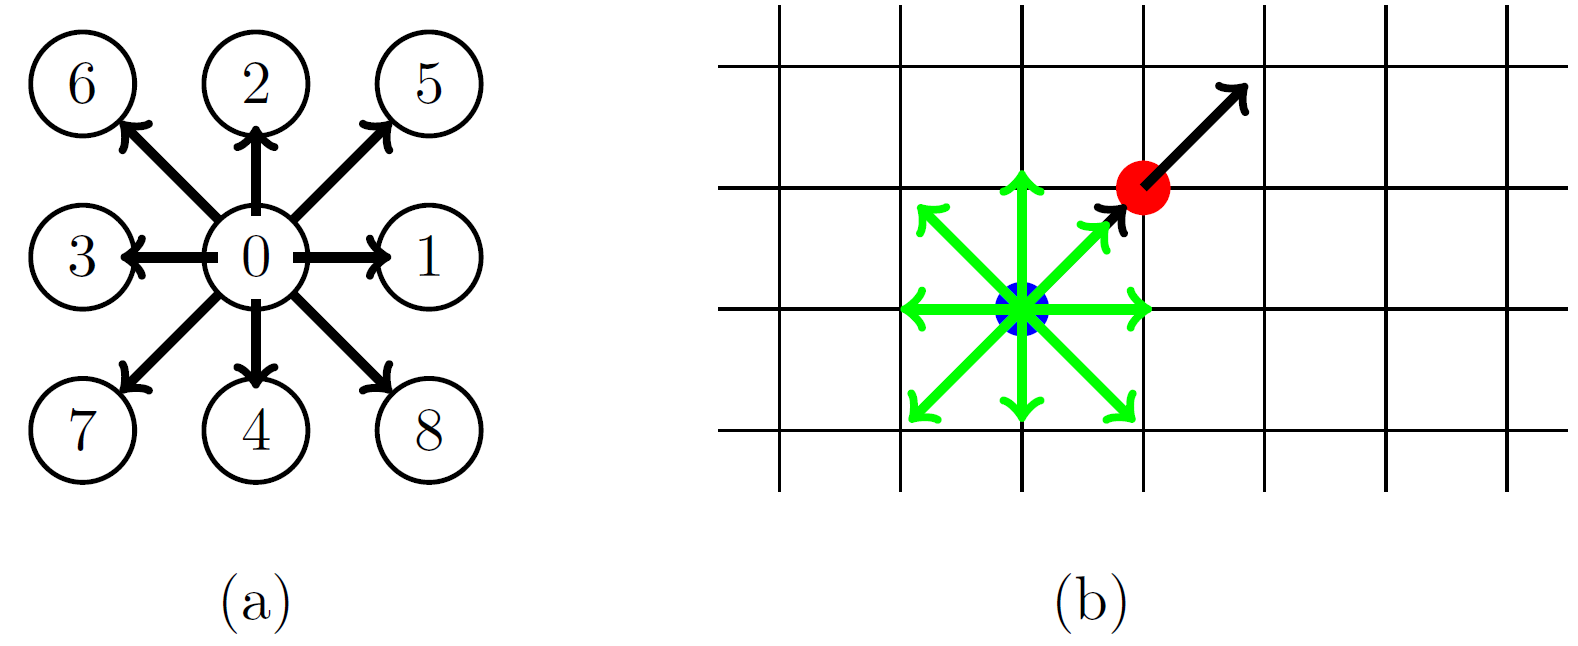
\includegraphics[width=10cm]{logos/Gitter_LBM.png}
   \caption{example figure}
  \label{fig:mesh}
  \end{center}
\end{figure}

\begin{algorithm}[tb]
  \caption{The name of Algorithm}
  \label{alg:label}
  \begin{algorithmic}[1]
    \Statex{$f$} \Comment{objective function}
    \Function{test}{}
    \For{$i= 0, 1, \dots$}
    \If{condition}
    \State{process} \Comment{comment}
    \EndIf
    \EndFor
    \EndFunction
  \end{algorithmic}
\end{algorithm}